\subsection{Implementation}

Formålet med dette afsnit er at gå fra vores design til kode.

\subsubsection{Søgning i krediteringer}%
\label{ssub:sogning_i_krediteringer}

Søgninger i krediteringer baserer sig på brugsmønster B03. Operationskontrakten
for dette brugsmønster ses i tabel \ref{tab:OperationsKontraktB03}. Det
udspecificerede sekvensdiagram ses på figur \ref{fig:B03OSDDesign}.

Fra \texttt{Menu.fxml} kaldes \texttt{submitSearch()} i controlleren
\texttt{MenuController}, ved tryk på søgeknappen. Hvis man kaster et blik på
MVC-modellen set på figur \ref{fig:mvc}, kan man at der her kaldes fra viewet i
\texttt{.fxml} filen til controlleren. \texttt{MenuController} sætter derpå et
nyt view, \texttt{SearchResult.fxml}. Dette view skal vise resultaterne af
søgningen. Dette ses i nedenstående snippet. Der sættes også en ny controller,
til at administrere det nye view.

\begin{lstlisting}
setContentPane("SearchResult.fxml", (Object) SearchController.getInstance());
SearchController.getInstance().setContent();
\end{lstlisting}

Derpå kalder \texttt{SearchController},

\begin{lstlisting}
SearchList.setItems(ApplicationManager.getInstance().search(searchString));
\end{lstlisting}

hvorpå at \texttt{ApplicationManager} i domænelaget står for at facilitere
søgningen, ved at kalde de korrekte Managers for at lave søgningen. Her bliver
\texttt{PersonManager} kaldt, hvorefter den kalder på \texttt{Factory}, som står
for kommunikationen med persistenslaget (ved at kalde
\texttt{DatabaseLoaderFacade}), for at de korrekte dataobjekter bliver
instantieret med den returnerede data. 

\begin{lstlisting}[basicstyle=\ttfamily\footnotesize, firstnumber=31,
label=lis:factory, caption=Forspørgsel til
persistenslaget og konstruktion af dataobjekter (\texttt{Factory.java})]
public ObservableList<IPerson> getPersons(String searchString) {
  ObservableList<IPerson> personObservableList 
    = FXCollections.observableArrayList();
    ResultSet personsResultSet 
        = DatabaseLoaderFacade.getInstance().searchPersonsFromDatabase(searchString);
    try {
        while (personsResultSet.next()) {
            IPerson tempPerson 
                = Mapper.getInstance().mapPerson(personsResultSet);
\end{lstlisting}

\texttt{DatabaseLoaderFacade}, kalder \texttt{DatabaseLoader} som queryer
databasen. Funktionen \newline\texttt{searchQueryToPersonList} har
\texttt{package-private}(som er standard) indkapsling. Således at dens
funktionalitet kan anvendes af \texttt{DatabaseLoaderFacade}, men ikke kan
tilgås udenfor pakken.

\begin{lstlisting}[basicstyle=\ttfamily\footnotesize, firstnumber=42,
caption=Query af databasen for personer (\texttt{DatabaseLoader.java})]
ResultSet searchQueryToPersonList(String searchString) {
  ArrayList<IPerson> personObservableList = new ArrayList<>();
  try {
    PreparedStatement queryStatement = getInstance().connection.prepareStatement(
      "SELECT * FROM credits, persons WHERE LOWER(name) LIKE LOWER(?) " +
        "AND credits.credit_id = persons.credit_id " /* +
        "AND jobs.person_id = persons.person_id " +
        "AND jobs.job_role_id = job_roles.job_role_id" */
    );
    queryStatement.setString(1, "%" + searchString + "%");
    queryStatement.executeQuery();

    return queryStatement.getResultSet();
\end{lstlisting}

Her i \texttt{DatabaseLoader} laves der en query til databasen, for personer
hvis navn ligner søgestrengen, samt hvilke jobs den fundne person har haft.

Resultatet af denne query (hvis den var succesfuld), returneres til domænelaget,
hvor \texttt{Factory} kalder \texttt{Mapper} (som tidligere set i
Listing~\ref{lis:factory}). \texttt{Mapper} tager et \texttt{ResultSet} og
returner en instans af \texttt{IPerson}. Dermed instantieres dataobjekter kun i
\texttt{Mapper}, således skjules instantieringen for resten af lagene.

\subsubsection{Implementering af Model-View-Controller mønsteret} 
%Hvordan sikrer gruppen at benytte sig effektivt af Model-View-Controller mønsteret?
\texttt{JavaFX}
libraryet indeholer en type af liste der kaldes \texttt{ObservableList}.  En
\texttt{Observablelist} fungerer som en almindelig \texttt{List<E>}, og kan
instantieres som bl.a. en \texttt{observableArrayList}. Det specielle ved en
\texttt{ObservableList} er at man kan tilføje en 'Listener'. En Listener er som
navnet angiver, en enhed der kan "lytte" efter ændringer på objekterne som
listerne indeholder. Lad os sige brugeren får præsenteret en liste af personer.
Dette er viewet i modellen. Her vælger brugeren så at godkende en person. Den
handling registrerer en controller (controller i mønsteret) og i programmet
kalder controlleren en funktion i \texttt{ApplicationManager}, der ændrer 
data nede i databasen (model i mønsteret). Da denne liste har en listener på
ændringer i data indeholdt i den pågældende \texttt{ObservableList}, notificrer
listener, som får viewet til at opdatere, så brugeren nu ser det opdaterede
data.  Tilføjelsen af en listener til en observableList er implementeret som
det ses på Listing \ref{lst:setContent}.

\begin{lstlisting}[language=Java, firstnumber=100, label=lst:setContent, caption = Funktionen
setContet sætter listen og hvordan denne opdateres]
private void setContent(AnchorPane listToApprove, ObservableList<? extends ICredit> creditList){
    int offset = 20;
    for (ICredit credit : creditList){
        if (!credit.isApproved()) {
            addItem(listToApprove, credit, offset);
            offset += 30;
        }
    }
    creditList.addListener((ListChangeListener<ICredit>) change -> {
        int offset1 = 20;
        while (change.next()) {
            if (change.wasAdded()) {
                for (ICredit credit : change.getAddedSubList()){
                    if (!credit.isApproved()){
                        addItem(listToApprove, credit, offset1);
                        offset1 += 30;
                    }
                }
            } else if (change.wasRemoved()) {
                for (ICredit credit : change.getRemoved()){
                    System.out.println("Removed credit: " + credit);
                    removeItem(listToApprove, credit);
                }
            }
        }
    });
\end{lstlisting}

Metoden \texttt{setContent} tager et \texttt{AnchorPane} og en
\texttt{ObservableList} som argumenter. Først tjekkes de \texttt{ICredit} som
listen indeholder igennem, og hvis de ikke er godkendt/approved bliver de
tilføjet til det medfølgende \texttt{AnchorPane}, som skal indeholde de krediteringer som
ikke er godkendt. Når der er itereret over alle krediteringer i listen, bliver
der tilføjet en listener til listen som starter ved linje 108 i listing
\ref{lst:setContent}. Listeneren lytter efter to ting. Om der bliver tilføjet
til listen, linje 111, og om der bliver fjernet fra listen, linje 118. Hvis der
bliver tilføjet til listen, tilføjes det nye element automatisk til det
\texttt{AnchorPane} som methoden har taget som argument. Hvis der fjernes fra listen,
fjernes dette element fra dette \texttt{AnchorPane}.

\subsubsection{GUI}%
\label{ssub:gui}

Systemets GUI eller graphical user interface er defineret i \texttt{.fxml}
filer. Disse sætter rammerne for hvad der vises på skærmen. Disse kan også
omtales som View i Model-View-Controller-modellen. Viewet kalder
funktioner i den controller der hører til viewet. Controlleren står for forsyne
viewet med data, dette gøres fx med \texttt{ObservableList} som tidligere nævnt.

En controller kan også på starttidpunktet for et view programmatisk indsætte
elementer i viewet. 

\paragraph{Menu}

\texttt{Menu.fxml} fungerer som en form for vindue-i-vinduet. Dette er da de
fleste views bliver vist inde i et \texttt{AnchorPane} i \texttt{
Menu}. Dette bevirket at man altid har adgang til søgemenuen og adgang til de
andre funktioner ens brugerniveau tilbyder. 

Dette ses fx her:
\begin{figure}[H]
    \centering
    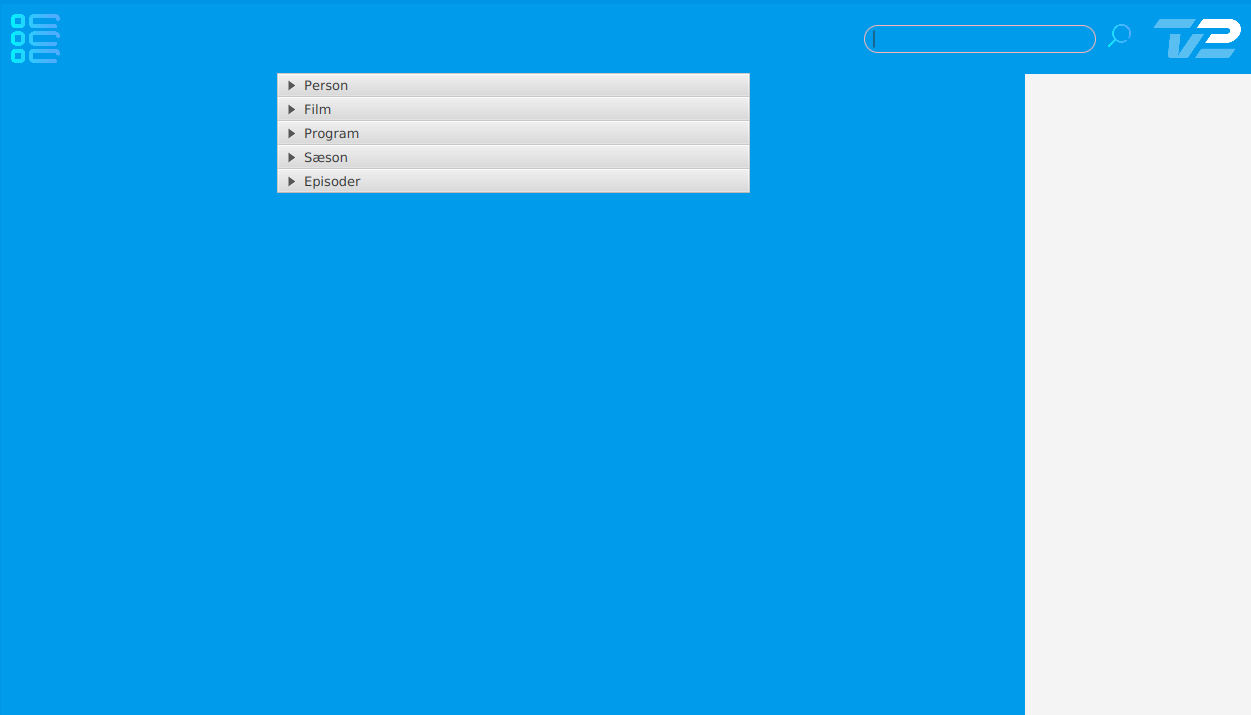
\includegraphics[width=0.7\textwidth]{images/menu.png}
    \caption{Menu, med et vindue inden i}
\end{figure}

her ses det at man kan godkende en krediteringer i mens der stadig er adgang til
hovedmenuen og søgefeltet.
